\section{Lempel-Ziv II: LZ78}
\label{sec:04}


\subsection{LZ78}

\paragraph{Basic idea} The \Define{LZ78} method does not use any search buffer, look-ahead buffer, or sliding window. Instead, it simply keeps a dictionary of previously encountered strings. The dictionary starts with the empty string at position zero and its size is only limited by the memory size.

The encoder outputs \Important{two-field tokens} (instead of three-field tokens in LZ77). Each token simply corresponds to a new string in the dictionary: it is of the form
\[
    (i, x),
\]
where $i$ is the position of the longest match in the dictionary and $x$ is the final character of the string.

Nothing is ever deleted from the dictionary:
\begin{itemize}
    \item Advantage over LZ77: future strings will be compressed even if they only match strings in the distant past;
    
    \item Drawback: the dictionary can become very large!
\end{itemize}

\paragraph{Example} Once again, it is best explained via a simple example. Say we want to compress
\begin{quote}
    sir\textvisiblespace sid\textvisiblespace eastman\textvisiblespace easily%\textvisiblespace teases\textvisiblespace sea\textvisiblespace sick\textvisiblespace seals
\end{quote}

The tokens are then (in order!):\\
~\\
\begin{tabular}{l|l|l}
     Dictionary position    & String    & Token  \\
     \hline
     0                      &  $\epsilon$         &        \\
     1                        & s           &  (0, s)      \\
     2                   & i          & (0,i)       \\
     3                   &  r         & (0,r)       \\
     4                   &  \textvisiblespace         & (0,\textvisiblespace)       \\
     5                   &  si         &    (1,i)    \\
     6                   &  d         & (0,d)       \\
     7                   &  \textvisiblespace e         &  (4,e)      \\
     8                   &  a         & (0,a)       \\
     9                   &  st         &    (1,t)    \\
     10                   & m          &    (0,m)    \\
     11                   & an          &   (8,n)     \\
     12                   & \textvisiblespace ea          & (7,a)       \\
     13                   & sil          &  (5,l)      \\
     14                   & y          &    (0,y)    
\end{tabular}
~\\
And the compressed output is the list of tokens
\begin{quote}
    (0,s) (0,i) (0,r) (0,\textvisiblespace) (1,i) (0,d) (4,e) (0,a) (1,t) (0,m) (8,n) (7,a) (5,l) (0,y)
\end{quote}

Once again, the decoder sees these tokens as ``instructions.'' But following these instructions means searching in the dictionary. A useful data structure for the dictionary is a \Important{tree}, where the root is the empty string and a new string is added to the tree as a child of the string it refers to on its token. Such a tree is called a \Define{trie}.

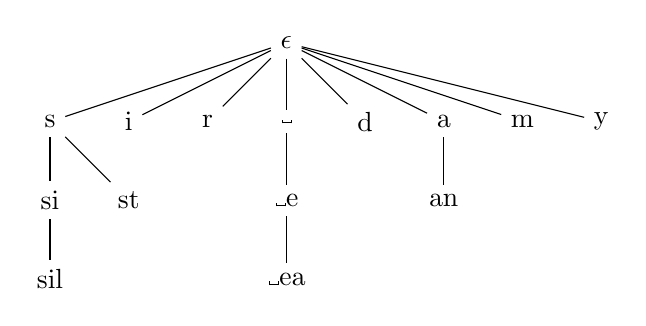
\begin{tikzpicture}
    \node (0) at (3,0) {$\epsilon$};
    
    \node (1) at (0,-1) {s};
    \node (2) at (1,-1) {i};
    \node (3) at (2,-1) {r};
    \node (4) at (3,-1) {\textvisiblespace};
    \node (5) at (0,-2) {si};
    \node (6) at (4,-1) {d};
    \node (7) at (3,-2) {\textvisiblespace e};
    \node (8) at (5,-1) {a};
    \node (9) at (1,-2) {st};
    \node (10) at (6,-1) {m};
    \node (11) at (5,-2) {an};
    \node (12) at (3,-3) {\textvisiblespace ea};
    \node (13) at (0,-3) {sil};
    \node (14) at (7,-1) {y};
    
    \draw (0) -- (1);
    \draw (0) -- (2);
    \draw (0) -- (3);
    \draw (0) -- (4);
    \draw (1) -- (5);
    \draw (0) -- (6);
    \draw (4) -- (7);
    \draw (0) -- (8);
    \draw (1) -- (9);
    \draw (0) -- (10);
    \draw (8) -- (11);
    \draw (7) -- (12);
    \draw (5) -- (13);
    \draw (0) -- (14);
    
    
\end{tikzpicture}



\subsection{LZW}


\paragraph{Basic idea} Lempel-Ziv-Welch (\Define{LZW}) is a variant of LZ78, with two main differences.
\begin{enumerate}
    \item The dictionary is \Important{initialised with all possible characters}. If we are compressing an ASCII file, then positions 0 to 255 are filled at initialisation.
    
    \item The tokens only have \Important{one field}! Since we always work with at least one character (that can always be found in the dictionary), there is no need to output the next character.
\end{enumerate}

Let us go back to our example:
\begin{quote}
    sir\textvisiblespace sid\textvisiblespace eastman\textvisiblespace easily%\textvisiblespace teases\textvisiblespace sea\textvisiblespace sick\textvisiblespace seals
\end{quote}

The dictionary is initialised with all 256 ASCII characters in positions 0 to 255, e.g. a is in position 97, b in 98, s in 115, z in 122. The first character in the string is s (in the dictionary at position 115). Since si does not appear in the dictionary, we add si to the dictionary at 256, and we continue with the character i. Again, since ir is not in the dictionary, we add ir at 257 and continue with the character r.

The dictionary (omitting positions 0 to 255) and the tokens look like this:\\
~\\
\begin{tabular}{l|l|l|l}
     Position & String & Token & What the token encodes \\
     \hline
     256 & si & 115 & s\\
     257 & ir & 105 & i\\
     258 & r\textvisiblespace & 114 & r\\
     259 & \textvisiblespace a & 32 & \textvisiblespace\\
     260 & sid & 256 & si\\
     261 & d\textvisiblespace & 100 & d\\
     262 & \textvisiblespace e & 32 & \textvisiblespace\\
     263 & ea & 101 & e\\
     264 & as & 97 & a\\
     265 & st & 115 & s\\
     266 & tm & 116 & t\\
     267 & ma & 109 & m\\
     268 & an & 97 & a\\
     269 & n\textvisiblespace & 110 & n\\
     270 & \textvisiblespace ea & 262 & \textvisiblespace e\\
     271 & asi & 264 & as\\
     272 & il & 105 & i\\
     273 & ly & 108 & l\\
        &   & 121 & y
\end{tabular}
~\\~\\
The output is then
\[
    115, 105, 114, 32, 256, 100, 32, 101, 97, 115, 116, 109, 97, 110, 262, 264, 105, 108, 121
\]

The dictionary can once again be stored as a tree, but the implementation is more complex than for LZ78. A thorough description is given in \cite[3.13.2]{Sal04}.


\subsection{Applications of LZW}

\paragraph{GIF} The ubiquitous Graphics Interchange Format (\Define{GIF}) uses a variation of LZW. It uses a dynamic, growing dictionary. It starts with the number of bits per pixel $b$: $b=2$ for monochromatic images, $b=8$ for an image with $256$ colours of shades of grey. The dictionary starts with $2^{b+1}$ entries and is doubled in size every time it fills up until it reaches $2^{12} = 4,096$ entries. At that point, the encoder may want to start a new dictionary!

GIF is not actually that good at image compression because it is unidimensional. It scans the image row after row, so it can detect similarities within a row but has trouble dealing with similarities across rows instead.

\paragraph{Limitations} One major issue of using LZW (e.g. for GIF), is that LZW is \Important{patented}. In response to that, the Portable Network Graphics format was created in the mid-90s (finalised in 96). It is based on DEFLATE (and hence LZSS) instead.

Another application of LZW was the Unix shell compression utility \texttt{compress}, that was used in the 80s. However, it was superseded by \texttt{gzip}, which typically outperforms it in terms of compression ratio.

\subsection{See further}

\paragraph{Variants} LZ78 and LZW also have a few variants, notably LZMW, LZAP and LZY. Have another look!

\paragraph{Kolmogorov complexity} The principle of Lempel-Ziv encoding is to construct a list of instructions to the decoder of the form ``Copy that string (and add that character).'' But what if we allowed any sort of instructions?

The \Define{Kolmogorov complexity} is a concept that predates Lempel-Ziv. It aims at evaluating the ``intrinsic'' complexity of a binary string. Simply put, the Kolmogorov complexity of a string $x$ w.r.t. a Turing machine $U$, denoted $K_U(x)$, is the shortest length of a program for $U$ that prints out $x$ and halts. Obviously, $K_U(x)$ is not computable. But still, we can say a lot about the Kolmogorov complexity of a random string: it's about the length of the string. Therefore, almost any string is incompressible! The study of Kolmogorov complexity and associated concepts (e.g. Solomonoff's universal probability or Chaitin's Omega number) is very intriguing but outside the scope of this course.



 \subsection{Exercises}

\begin{exercise}
Encode the string
\begin{quote}
    sir\textvisiblespace sid\textvisiblespace eastman\textvisiblespace easily\textvisiblespace teases\textvisiblespace sea\textvisiblespace sick\textvisiblespace seals
\end{quote}
with LZ78: give the dictionary table, the trie, and the output.

Encode the same string with LZW.
\end{exercise}


\begin{exercise}
Select a few (small) images, and compare the file sizes for those when saved as .bmp, .gif and .png.
\end{exercise}














unsigned char ucDataBlock[16] = {
	// Offset 0x00000000 to 0x00000015
	0x42, 0x0D, 0x0D, 0x0A, 0x00, 0x00, 0x00, 0x00, 0x7A, 0x4E, 0x25, 0x5A,
	0x68, 0x30, 0x00, 0x00
}








